\chapter{Concept}
The application should be accessible to all employees of SinnerSchrader. Due to the heterogeneity of the the users' computer setups running \textit{Windows}, \textit{macOS} and \textit{Linux}, creating a native application supported by everyone’s system is a rather complicated task. A web application using standard technologies does not only solve this problem, but can also be used from mobile devices such as smart phones and tablets. Furthermore, there is no need to manually install and update the software so that it can be assumed that all users use the latest version of the application. This is a positive factor regarding the overall usability of the system and assures bugs and security issues are eliminated the moment a fixed version of the software is deployed. All those advantages compared to native clients and the fact that SinnerSchrader’s expertise lies in the development of web applications lead to the decision, that such an application would be the appropriate choice.

\section{Person Search}
The central feature of the application is the search function that returns a list of all persons matching the entered set of skills. By default, the results are ordered by a fitness score which describes how well a person matches into the set of searched skills. As a consequence of this sorting, the application implicitly recommends the best matching person to the user, thus it falls within the group of \textit{recommender systems}.

\subsection{Recommender Systems}
Recommender systems ``are information filtering systems that deal with the problem of information overload by filtering vital information fragment out of large amount of [...] information'' \cite{Isinkaye2015261}\label{recommender-definition} which are commonly used to recommend an item to the user based on their previous interactions with other items. For example, recommender systems are used to predict products a customer might want to buy based on the ones they already bought in order to present those items more prominentely than articles the customer is unlikely to buy. In this application's context, the recommender system will filter the set of all employees and recommend better results by showing them first.

\subsection{Techniques of Content Filtering}
As described by Isinkaye et al., filtering techniques used in recommender systems are divided in three classes: model based, memory based and hybrid. Each of this classes relies on a different approach for gaining data to filter the information by \cite{Isinkaye2015261}.

\subsubsection{Content Based Filtering}
	The content is filtered by examining its attributes in order to find items that are contentually similar to the one the user is currently or has previously been interacting with.
\subsubsection{Collaborative Filtering}
	Collaborative filtering techniques rely on the assumption that users can be divided into groups of \textit{neighbors} that behave similarly, so that reccommendations are decutable from ohter users' former interactions.
	\begin{itemize}
		\item Model Based Filtering\\
		Model based filtering applies methods of machine learning and data mining to learn a pre-computed model which predicts the users' interactions.
		\item Memory Based Filtering\\
		Memory based filtering techniques employ the saved interaction history and generate recommendations based on it. In contrast to model based filtering, memory based filtering does not learn a given model but operates directly on the known data.
		\begin{itemize}
			\item User Based Filtering\\
			The user's interactions with items are examied in order to find neighbors that share a similar activity history. Once neighbors are found, the system combines their interaction histories in order to find items to user is likely to appreciate getting recommended.
			\item Item Based Filtering\\
			Item based filtering combines all users' interactions and creates a model describing which items are similar to another. This model is then used to recommend items similar to the ones the user has given positive feedback for.
		\end{itemize}
	\end{itemize}
\subsubsection{Hybrid Filtering}
Hybrid filtering combines two or more filtering methods either by aggregating their respective results into a single set of recommendations preferring the items multiple methods recommend, or by bringing content based aspects into the approach of collaborative filtering and/or vice versa.

\subsection{Search Algorithm}
In the context of the search function, all employees are searchable items. Their attributes include name, location and their respective skills structured as pairs of skill level and will level. This data will be used in an content based filtering approach that not only finds suitable employees, but also ranks them by their fitting into the searched skill set. Other users' interactions with search results, for example the opening of a found person's profile, will not be taken into account, since there is no direct connection between these actions and the person's fitness. Furthermore, a system based on the user's former selections would be inadequate, because the application is meant to give managers the ability to find employees they did not already have contact with; recommending persons the searching user had interacted with would thus be counterproductive.

\subsubsection{Outline}
The basic structure of the search function will be:
\begin{enumerate}
  \item Create a list of all employees
  \item Filter by Skills\\
    Remove all employees from the list that do not have all skills the user searched for. At this point, only the presence of the skill in the employees' profiles is taken into account; skill/will levels are ignored.
  \item Filter by Location\\
    If the user specified a location to search for, remove all employees from the list that do not match it.
  \item Assign Fitness Scores\\
    Assign a fitness score to all remaining employees. This fitness score takes into account the user's skill/will levels and their specializations.
  \item Sort by fitness score\\
    The results will be sorted by fitness score. The employee with the best fitness score will be shown first in the list of results, so an implicit recommendation
    is made by the system.
  \item Return Results
\end{enumerate}

\subsubsection{Pseudo-Implementation}
\begin{figure}
\begin{lstlisting}[language=Java]
function search(searchItems, searchLocation) {
  var results = getAllEmployees()

  for (Employee e in results) {
    if (e.skills does not contain all elements of searchItems) {
      results.remove(e)
    }
  }

  for (Employee e in results) {
    if (e.location is not searchLocation) {
      results.remove(e)
    }
  }

  for (Employee e in results) {
    e.assignFitnessScore()
  }

  results = results.sortByFitnessScore()

  return results
}
\end{lstlisting}
\caption{Pseudo-Implementation of the search algorithm}
\end{figure}

\subsection{Scoring Algorithm}
\label{fitscorealg}
The application will sort all found persons by their fitness into the searched skill set; so there has to be an algorithm that can assign a score describing said fitness to every person.

\subsubsection{Requirements}
According to Spoonamore et al., an algorithm that matches persons to positions based on their skills has to meet more demands than solely the functional ones. They define the specific requirements such an algorithm assigning naval personnel to positions on a ship as follows:
\begin{itemize}
  \item Easy to implement and maintain
  \item Fast to execute, so as not to become a computational bottleneck
  \item Takes into account factors: rating, pay grade and NECs\footnote{Navy Enlisted Classifications} and future taxonomies characterizing required knowledge, skills and abilities
\end{itemize}\cite[P. 14]{USN}

\label{customizable}
These qualities include factors very specific to the US Navy and thus will have to be evaluated and traslated into SinnerSchraders field of operation, but general requirements such an algorithm has to meet can be deducted: It may not be too complex as employees must be able to understand the system they are rated by, it should take into account different groups of factors and must be easy to adjust in order to keep the system maintainable.

\subsubsection{Factors to Include}
An estimation of a concrete person's fitness into a position described by the searched skill set needs not only to take into account the matching of offered and required skills, but also the employees motivation to apply said skills derived from their preferences and their personal specialities and expertise. The latter can be described as the skill and will levels that are significantly higher than the person's average level. So the important factors to be included in the algorithm are:
\begin{itemize}
  \item Average level of knowledge regarding the searched skills.
  \item Average level of will regarding the searched skills.
  \item Specialization in the searched skills, including:
  \begin{itemize}
    \item Specialization in knowledge about the searched skills.
    \item Preference of the searched skills over others.
  \end{itemize}
\end{itemize}


\subsubsection{Proposed Fitness Score Algorithm}
Skill and will levels are described as integer values on a scale form zero to three. This scale, called $V$, can be expressed as
\begin{gather*}
  V = \{ x \in \mathrm{N}_0^+ \ | \  0 \leq x \leq 3\}
\end{gather*}

All existing skills are accumulated in the set $S$. The employee's skills are represented by $E$ which is a subset of $S$. The search items are
defined as $Q$.

\begin{gather*}
  S = \{java, ruby, ...\} \\
  E = \{x \in S \ | \ \textrm{employee has skill x}\} \\
  Q = \{x \in S \ | \ \textrm{user searches for skill x}\} \\
\end{gather*}

The functions $v_s$ and $v_w$ assign a level of skill/will to each value in $E$.
\begin{gather*}
  v_s: E \mapsto V \\
  v_w: E \mapsto V \\
\end{gather*}

The averages of the employees' skill/will values of the searched skills are defined as $a_s$ and $a_w$.
The variables $s_s$ and $s_w$ describe the employee's specialization in the searched items and are defined as the difference
of the average skill/will level of the searched items and the average level of all other items.
A person with maximal interest and knowledge in all searched items and an infinite number of skills with the minimal
value of zero would have the greatest specialization possible and thus get assigned a value of one.

\begin{gather*}
  a_s = \left( \sum_{x \in E \cap Q} v_s(x) \right) \cdot \frac{1}{|E \cap Q|} \\
  a_w = \left( \sum_{x \in E \cap Q} v_w(x) \right) \cdot \frac{1}{|E \cap Q|}
\end{gather*}
\begin{gather*}
  s_s = \frac{|V| \ + a_s - \left( \left( \sum_{x \in E \setminus Q} v_s(x)\right) \cdot \frac{1}{|E \setminus Q|} \right)}{2 \ |V|}\\
  s_w = \frac{|V| \ + a_w - \left( \left( \sum_{x \in E \setminus Q} v_w(x)\right) \cdot \frac{1}{|E \setminus Q|} \right)}{2 \ |V|}
\end{gather*}

The resulting fitness score $f$ is a weighted mean of the introduced facors. The weights $w_{as}$, $w_{aw}$, $w_{ss}$, $w_{sw}$ sum up to one.\footnote{Mathematically, this is not neccessary, but it results in much more human readable fitness score values between zero and one.}

\begin{gather*}
  f = \frac{w_{as} \cdot a_s}{|V|} + \frac{w_{aw} \cdot a_w}{|V|} + w_{ss} \cdot s_s + w_{sw} \cdot s_w \\
  w_{as} + w_{aw} + w_{ss} + w_{sw} = 1
\end{gather*}

\subsubsection{Example Caculation}
Let there be three example employees, Alice, Bob, and Charlie, having the same three skills each.
(Notation: skill level/will level)
\label{example-fitness}
\newline
\newline
\begin{center}
\begin{tabular}{r|ccc}
  Person  & Java & Ruby & C++ \\
  \hline
  Alice   & 2/1  & 2/2 & 3/3 \\
  Bob     & 2/3  & 0/3 & 0/1 \\
  Charlie & 3/3  & 2/1 & 1/2 \\
\end{tabular}
\end{center}

Applying the algorithm with $w_{as} = w_{aw} = w_{ss} = w_{sw} = 0.25$ to a search for the skills \textit{Java} and \textit{Ruby} results in the following values\footnote{Values have been rounded off to two significant digits.}:


\begin{center}
\begin{tabular}{r|ccccc}
  Person  & $a_s$ & $a_w$ & $s_s$ & $s_w$ & $f$\\
  \hline
  Alice   & 2   & 1.5 & 0.33 & 0.25 & 0.44\\
  Bob     & 1   & 3   & 0.67 & 0.83 & 0.71\\
  Charlie & 2.5 & 2   & 0.75 & 0.5  & 0.69\\
\end{tabular}
\end{center}

Ranking the employees only by the average value of skill regarding the two searched items would result in Charlie being preferred to Alice and Alice being preferred to Bob. Sorting them using the proposed fitness score, however, would result in Bob being recommended as the best match, because his relatively high interest in the searched skills and his specialization in them compensates his low average skill. Interestingly, Alice has the best average skill level but nonetheless gets scored the worst due to her obvious specialization in C++. In real life usage, the weighting constants $w_{as}$, $w_{aw}$, $w_{ss}$ and $ w_{sw}$ might need to be adjusted so that the average skill plays a bigger role in the resulting score.\footnote{The need to adjust the weights should not be considered a design flaw, since the algorithm has been intentionally designed to be customizable to the users' needs as defined in \ref{customizable}.}

\subsection{Example Search}
For this example, let the set of employees be Alice, Bob, Charlie, Donald, and Erika, and the set of all known skills be Java, Ruby, and C++.
The assignment of skill/will levels and the respective locations are:
\newline
\begin{center}
\begin{tabular}{r|c|ccc}
  Person  & Location & Java & Ruby & C++ \\
  \hline
  Alice   & Hamburg   & 2/1 & 2/2 & 3/3 \\
  Bob     & Hamburg   & 2/3 & 0/3 & 0/1 \\
  Charlie & Hamburg   & 3/3 & 2/1 & 1/2 \\
  Donald  & Hamburg   & 3/3 &  -  & 2/2 \\
  Erika   & Frankfurt & 1/1 & 2/3 & 3/1 \\
\end{tabular}
\end{center}

Applying the algorithm and searching for employees knowing Java and Ruby in Hamburg:\\
(Let the weights used in the fitness score be $w_{as} = w_{aw} = w_{ss} = w_{sw} = 0.25$)
\begin{itemize}
  \item Create a list of all employees\\
    $\Rightarrow$ Alice, Bob, Charlie, Donald, Erika
  \item Filter by skills: Donald gets eliminated because he does not have the skill \textit{Ruby}\\
    $\Rightarrow$ Alice, Bob, Charlie, Erika
  \item Filter by location: Erika works in Frankfurt and thus will be excluded\\
    $\Rightarrow$ Alice, Bob, Charlie
  \item Assign fitness scores\footnote{The calculation of the fitness scores can be seen in \ref{example-fitness}}\\
    $\Rightarrow$ Alice (0.44), Bob (0.71), Charlie (0.69)
  \item Sort by fitness score\\
    $\Rightarrow$ Bob (0.71), Charlie (0.69), Alice (0.44)
\end{itemize}



\section{Search Suggestions}
After entering an item into the search bar, the user will be presented other items they are likely to enter next. This minor feature can be seen as another
recommender system, because it recommends the next item from the set of all available search items and thus matches the definition given in \ref{recommender-definition}. This recommender system has to deal with other limitations than the one used for the main search function. It filters a completely different set of data, namely all skills instead of all persons, and uses a different filtering approach.

\subsection{Available Data}
\subsubsection{Distinguishable Users}
Since it is not planned that users will have to log in before performing a search,
there is no user context that can be used examine a person's former interactions
in order to predict their next ones and recommending it.\\
As the system is designed to be a web application, a cookie holding an unique identifier could be stored on the client device. The application would then use this ID to aggregate interactions made by the same person. Unfortunally, this method cannot itentify a known person using another device as multiple devices will not share the same ID. Furthermore data collected about a user will be discarded if they delete their devices cookies or change browsers.
This approach would also need the application to inform the user that data will be stored on their devices as stated by Article 15(3) of the Telemediengesetz (TMG). The user has to give their approval and must be able to refuse the saving of their data (BDSG, Section 4a).\\
There also exist various methods to identify users without the need to store any data on their devices by examining and recognizing their devices attributes. The collected data can include
factors like language settings, the used browser and its version, and the devices hardware components. All this data combined can be used to form an almost unique fingerprint which can be used to recognize a device \cite{finger}.\\
Another possibile method would be to recognize users by examining their very own usage behaviour such as typing patterns or mouse strokes. This approach called \textit{user fingerprinting} does not depend on the users device and thus can be used to identify people across multiple devices and browsers. On the downside, this method can only differntiate between users typing the same word and needs a multitude of samples of each user in order to be able to recognize them \cite{typing}.
Although device and user fingerprinting is not prohibited by law,
the \textit{Opinion 9/2014 on the application of Directive 2002/58/EC to device
fingerprinting} by the EU's \textit{Article 29 data protection working party} states that a user must be informed about the fingerprinting process and be able to deny this.
To sum up, the described methods to identify unique persons create an exorbitant computational effort and/or have high error rates for not being able to determine a single user across multiple devices. For the further design of the skill search recommender system, it will be assumed that there is no data about unique users, but about their entirety.

\subsubsection{Skill Attributes}
The skills are planned to be saved as simple names not enriched with any metainformation, so using content based filtering is not a trivial task. One possible approach would be to use linguistic methods to find similarities in names of skills in order to form clusters of related skills. Unfortunally, most of the skills' names are arbitrarily chosen or acronyms, so that this form of analysis will fail to detect any menaingful attributes.\\
Regarding the concept of the suggestion engine, the assumption is made, that there is no context to the skills and that the only information about any skill is its name.

\subsubsection{Aggregated Search History}
Tracking which skills have been searched together can be implemented easily and creates a fair amount of data to generate potentially useful suggestions. Legally, this is not problematic if the application does neither save personal data about the users (Article 15 Telemediengesetz), nor stores information that could potentially be used to create personal usage profiles that can be matched to specific persons (Article 15(3) Telemediengesetz). Grouping skills that have been searched jointly does not stand in conflict with those regulations and requires no information about distinguishable user, so the application will store the search history.

\subsection{Choosen Appoach}
Assmuning that no user profiles exist, user based filtering and model based filtering cannot be applied. Due to the lack of metadata about the skills, content based filtering can also be eliminated as a possible approach. Item based filtering, however, does not require any data that is not available, so this approach will be used for the recommender system.

\subsection{Concept}
The application has access to the list of skills the user already entered and to a repository of all previous searches. Having this information, the system will use a markov chain to predict the next item that the user is likely to entered and recommed it to them.

\subsubsection{Markov Chains}
Markov chains are a relatively simple tool for predicting future states of systems based on the current state. In fact, makrov chains rely on the fact, that the next state of the system is only dependent on the current state, which is called the \textit{markov property} \cite{markprop}. In the context of the skill management application, we assume this to be true because only two states will be examined: the current state is represented by the set of all items entered in the search field; the future state is skill set of the current search plus one more item.
The basic concept is to store all possible states of the system and the respective probability of switching between from any state to any other one.
Knowing the current state one can easily deduct the most probable future state. When a state transistion occurs, the outgoing probabilities of the origin states
can be adjusted accordingly in order to factor the transition into the prospective projections.
\begin{figure}[!htp]
    \centering
    \includegraphics[width=0.33\textwidth]{images/markov-chain.png}
    \caption[Markov Chain]{A simple markov chain displayed as graph. The states are represented as vertices. All possible transitions between states are denoted as edges. The edge weights define the probability of the transition relative to all other outgoing edges of a node.}
    \label{fig:markovchain}
\end{figure}

\subsubsection{Data Structure and Algorithm}
In order to get the best results, the recommender system should save all combinations of items that have previously been searched for together and then recommend
the next one based on this exact starting point. On the downside, this would result in a lot of different origin states that contain very few possible future states due to being to
specific to a single search. The stored data can only be used if the exact same combination of skills is entered again.\\
Another way to implement such a recommendation system would be to only inspect the last entered search item and ignoring all other ones. Given $n$ known skill items, all probabilities for the future state could be saved in one single $n \times n$ matrix saving only $n^2$ values.
This solution would disregard the whole context of the search item.\\
As a tradeoff, the system will generate predictions for each skill in the search query independently and aggretage these predictions afterwards. For each skill, a list of possible recommendations paired with the total count of searches for both will be stored. The recommendation lists of all skills combined represent the transition matrix. Instead of transition probabilities, the total number of searches is saved in order to simplify the aggreation of multiple suggestions.\\
The recommender system will concatenate the suggestion lists of all items in the current search query and add up the counts of skills appearing in multiple suggestion lists. Then, all elements of the combined list that are part of the search query will be removed, the result is a list of suggestions for the whole search query.\\

\newpage
\subsection{Pseudo-Code}
\begin{figure}
\begin{lstlisting}[language=Java]
var knownSkills = [
  {
    name: "java",
    similar: [
      {
        name: "php",
        count: 3
      }, {
        name: "ruby",
        count: 2
      }
    ]
  }, {
    name: "php",
    similar: [
      {
        name: "java",
        count: 5
      }, {
        name: "ruby",
        count: 2
      }
    ]
    name: "ruby",
    similar: [
      {
        name: "java",
        count: 0
      }, {
        name: "php",
        count: 5
      }
    ]
  }
]
\end{lstlisting}
\caption[Skill Data Structure (Pseudo-Implementation)]{Pseudo-Implementation of the known skills' data structure}
\end{figure}

\newpage

\begin{figure}
\begin{lstlisting}[language=Java]
function suggest(searched) {
  var accumulated = {};

  for (s in searched) {
    for (t in knownSkills.getByName(t).getSkillsSearchedWith()) {
      if (accumulated.getByName(t) exists) {
        accumulated.getByName(t).count += t.count
      } else {
        accumulated.getByName(t) = t.clone()
      }
    }
  }

  for (t in accumulated) {
    if (searched contains t) {
      remove t from accumulated
    }
  }

  return accumulated.getHighestCount();
}

\end{lstlisting}
\caption[Skill Suggestion Algorithm (Pseudo-Implementation)]{Pseudo-Implementation for the suggestion of a known skill based on a set of already searched items}
\end{figure}

\subsection{Example}
Transition Matrix:

\begin{center}
\begin{tabular}{c | c |c | c | c}
		  & Java & PHP & CSS & COBOL\\
	\hline
	Java  &  -   &  7  &  3  &   1  \\
	\hline
	PHP   &  7   &  -  &  9  &   5  \\
	\hline
	CSS   &  3   &  9  &  -  &   8  \\
	\hline
	COBOL &  1   &  5  &  8  &   -  \\
\end{tabular}
\end{center}

Using the given transition matrix and the seaerch query ``Java, PHP'', the algorithm works like this:
\begin{enumerate}
	\item Retrieve suggestion lists for each search item\\
		$\Rightarrow$ PHP (7), CSS (3), COBOL (1), Java (7), CSS (9), COBOL (5)
	\item Aggregate lists (combine counts)\\
		$\Rightarrow$ PHP (7), Java (7), CSS (12), COBOL (6)
	\item Remove suggestions that are part of the search query\\
		$\Rightarrow$ CSS (12), COBOL (6)
	\item Suggest item with the highest total count\\
		$\Rightarrow$ CSS
\end{enumerate}

\begin{figure}[!htp]
    \centering
    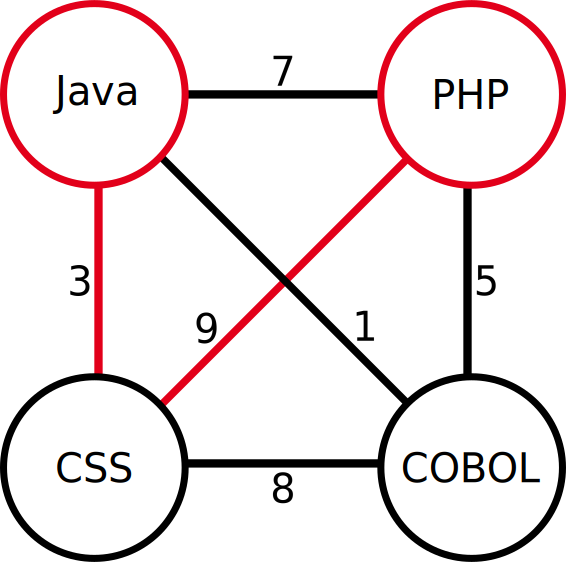
\includegraphics[width=0.33\textwidth]{images/markov_impl.png}
    \caption[Search Suggestion Markov Model]{Markov Model used in the example. The two origin states and the transitions that form the end result are highlighted red.}
    \label{fig:wireframe}
\end{figure}

\section{Visual Concept \& Wireframes}
The application should be as simple as possible and usable for everyone, in order to provide an efficient and fast tool. Thus, it will be designed as a single page application based around a people search that provides a way to input the skills needed and returns all persons offering said skills. After entering a search, the user can select any of the found colleagues and view their personal profile showing extended information like contact details, more skills the user did not search for, and the employee's location. This profile will also include links to directly contact the inspected person via Email or Google Hangouts\footnote{https://support.google.com/hangouts/answer/2944865}. Unlike the considered commercial solutions (see \ref{commercial}), this tool will not include features like creating statistics, assessments, applicant management, or any dashboard other than the basic search view.
Furthermore, there will not be any different roles with different access rights for employees and their managers, since this application is meant to be a tool enhancing collaboration, not supervision.
\begin{figure}[!htp]
    \centering
    \includegraphics[width=\textwidth]{images/wireframe.png}
    \caption[Search Result Page (Wireframe)]{Wireframe of the search result view}
    \label{fig:wireframe}
\end{figure}

\begin{figure}[!htp]
    \centering
    \includegraphics[width=\textwidth]{images/design_home.png}
    \caption[Search Page (Concept)]{An early prototypical designs for the search view}
    \label{fig:design_home}
\end{figure}

\section{Legal Concerns}
Nearly all of data fall into the category of personal data (\textit{Personenbezogene Daten}), which is defined as ``any information concerning the personal or material circumstances of an identified or identifiable individual (the data subject)'' (BDSG, 3(1)). The personal data will be collected (BDSG, 3(3)), processed (BDSG, 3(4)) and transfered (BDSG, 3(3)) to other employees of SinnerSchrader.
Generally, this does not violate any law, since the ``collection, storage, modification or transfer of personal data or their use as a means of fulfilling one’s own business purposes shall be admissible'' (BDSG, 28(1)), but some restrictions apply: the data subjects have to be informed about the processing of their personal data, must be able to deny their consent (BDSG, Section 4a), and the personal data shall not be made public.
To ensure the latter, the application must not be accessible to persons that do not work for or on behalf of SinnerSchrader. Technically, this will be arragned by making the application attainable from SinnerSchrader's internal network only, which can only be used by employees and authorized persons.

TODO: Betriebsrat
